\documentclass[12pt]{article}

\usepackage{fullpage}
\usepackage{graphicx, rotating, booktabs} 
\usepackage{times} 
\usepackage{natbib} 
\usepackage{indentfirst} 
\usepackage{setspace}
\usepackage{grffile} 
\usepackage{hyperref}
\usepackage{adjustbox}
\setcitestyle{aysep{}}


\singlespace
\title{\textbf{Appendix: Does U.S. Success Promote Democracy Abroad?}}
%\author{Joshua Alley and John Owen} 
\date{}

\bibliographystyle{apsr}

\begin{document}

\maketitle 

\singlespace 

This appendix provides more detail about the multilevel models and an extension with varying slopes at the individual level. 
Please note that the World Values survey does not permit disseminating copies of the data in replication archives. 
We used version 1.6 of the World Values survey longitudinal data, which can be downloaded from: \url{https://www.worldvaluessurvey.org/WVSDocumentationWVL.jsp}. 


\section{Model Specification} 

\subsection{Fixed Year-Level Slopes} 

The binomial likelihood of the proportion of high democratic support across the number of respondents within each state-year group can be expressed as follows, with the probability of success $\theta$ in each country-year observation partially pooled such that ~ $\theta_i \sim N(\mu_i, \sigma)$ : 

\begin{equation}
\mathrm{ y \sim Binomial(Num. Resp, \theta)}
\end{equation} 


The expected value of high democratic support $\mu$ in each state-year observation is:
\begin{equation}
\mathrm{\mu_i = \alpha + \alpha_{state} + \alpha_{year} + \textbf{X} \beta + \textbf{Z} \gamma}
\end{equation}

Then the year level variables predict the mean of each year varying intercept in a regression model with a constant term. 

\begin{equation}
\mathrm{\alpha_{year} = \textbf{G} \lambda }
\end{equation}

\autoref{tab:priors} summarizes the prior distributions in the multilevel model. 
All priors are weakly informative relative to the scale of the data, and the regression parameters are robust to unusually large effect sizes. 
We employ non-centered parameterizations of the state and year intercepts in fitting the model. 

\begin{table} % Create a table of priors.
\begin{center}
\begin{tabular}{c} 
$ p(\alpha) \sim N(0, 1)$  \\
$ p(\alpha_{year}) \sim N(G \lambda, \sigma^{yr}) $ \\ 
$ p(\sigma^{yr}) \sim \mbox{half-}N(0, 1) $ \\
$ p(\alpha_{state}) \sim N(\mu_{state}, \sigma^{st}) $ \\ 
$ p(\mu_{state}) \sim N(0, 1) $ \\ 
$ p(\sigma^{st}) \sim \mbox{half-}N(0, .5) $ \\ 
$ p(\beta) \sim \mbox{student-t}(5, 0, 1) $ \\
$ p(\gamma) \sim \mbox{student-t}(5, 0, 1) $ \\
$ p(\lambda) \sim \mbox{student-t}(5, 0, 1) $ 
\end{tabular} 
\caption{Summary of Priors in Multilevel Model} 
\label{tab:priors}
\end{center} 
\end{table} 

Given these priors, the regression model can be rewritten as: 
\begin{equation}
\mathrm{ \mu = \alpha + \alpha_{state} + N(G \lambda, \sigma^{yr}) + \textbf{X} \beta + \textbf{Z} \gamma)}
\end{equation} 

We express the varying slopes model with this alternative notation, as it makes indexing by region more straightforward. The next section summarizes the varying slopes model. 

\subsection{Varying Year-Level Slopes} 

The varying slopes model lets the relationship between U.S. success and other year-level factors shift across states, rather than assuming a constant effect. 

\begin{equation}
\mathrm{ \mu = \alpha + \alpha_{state} + \alpha_{year} + \textbf{X} \beta + \textbf{Z} \gamma +  \textbf{G} \lambda_{region}} 
\end{equation} 

The specification subsumes regional intercepts and state-year varying slopes into a multivariate normal prior with covariance matrix $\Sigma$ with an LKJ prior, further optimized with a Choleskey factorization: 

\begin{equation}
\mathrm{\alpha_{region}, \lambda_{region} \sim \mbox{multivariate normal}(\mu_{region}, \mu_{\lambda}, \Sigma)}
\end{equation}


\section{Hamiltonian Monte Carlo Diagnostics}

We fit these models with STAN \citep{Carpenteretal2016}.
There were no divergent iterations in either sample running 4 chains for 2,000 iterations with 1,000 warmup iterations in any of the imputed datasets.  
The split $\hat{R}$ statistic is less than 1.1 for all parameters as well.
Energy diagnostics and the effective sample size for the potsterior medians and tails were also satisfactory.  
All of these estimates suggest that the Hamiltonian Monte Carlo adequately explored the posterior distribution. 


\begin{figure}
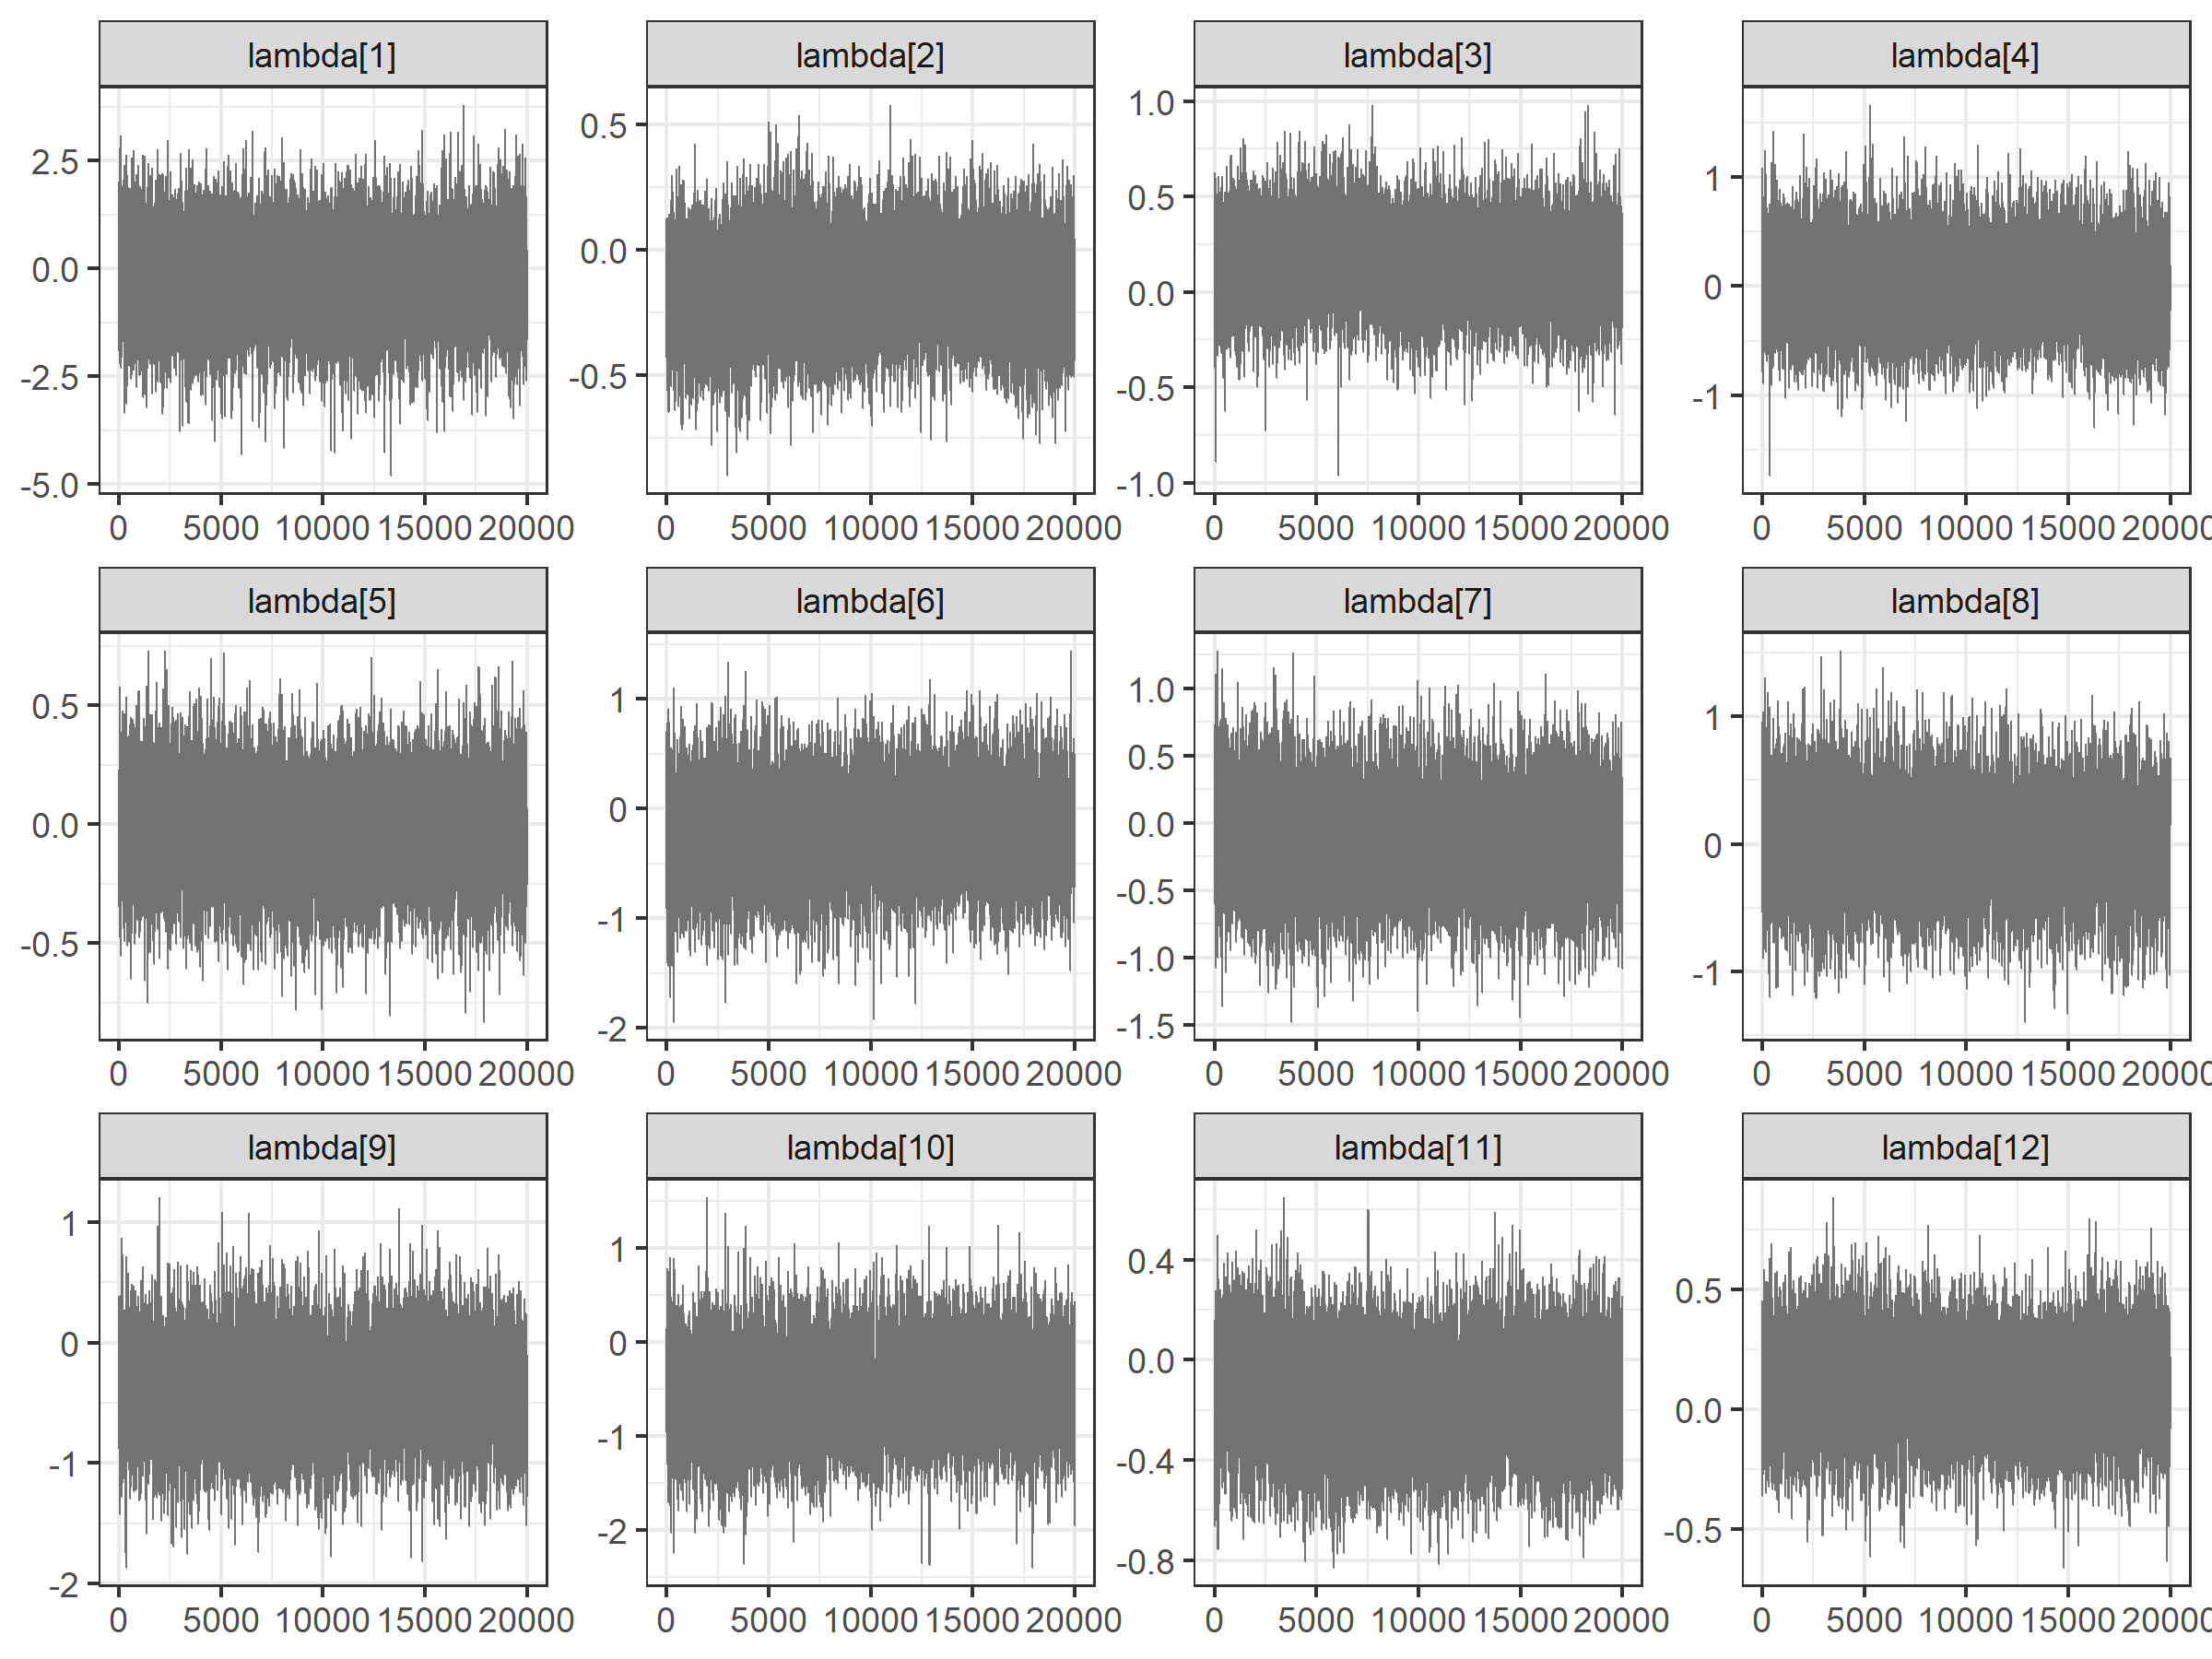
\includegraphics[width = .95\textwidth]{lambda-trace.png}
\caption{Trace plot of the year-level regression parameters in a multilevel model of foreign attitudes towards democracy and U.S. success, 1980 to 2019.}
\label{fig:lambda-trace} 
\end{figure}

\section{Variables}


This section summarizes the key variables in the model. 
We start with the year-level variables that measure U.S. success and failure. 
\autoref{tab:year-vars} summarizes these variables and their distribution. 
\autoref{tab:state-vars} summarizes the state-level variables across all imputed datasets.
Last, \autoref{tab:wvs-vars} shows summary statistics for the individual level variables in the analysis, which are averaged at the state year. 
It also includes the distribution of high democratic support sums and the number of respondents, which are the key quantities in the binomial proportions.
 
 
\begin{table}
\caption{\label{tab:year-vars}Year Level Variables}
\centering
\begin{tabular}[t]{lrrrrrrr}
\toprule
  & Unique (\#) & Missing (\%) & Mean & SD & Min & Median & Max\\
\midrule
US GDP Growth & 29 & 0 & 2.58 & 1.66 & -2.54 & 2.68 & 4.75\\
US Democracy & 23 & 0 & 0.80 & 0.03 & 0.74 & 0.80 & 0.86\\
US Human Rights & 29 & 0 & 0.73 & 0.68 & -0.17 & 0.55 & 1.88\\
US Protests & 29 & 0 & 0.69 & 0.17 & 0.42 & 0.72 & 1.05\\
US GINI & 22 & 0 & 36.72 & 1.93 & 31.60 & 37.40 & 38.50\\
Republican Pres & 2 & 0 & 0.48 & 0.51 & 0.00 & 0.00 & 1.00\\
Trump Pres & 2 & 0 & 0.07 & 0.26 & 0.00 & 0.00 & 1.00\\
Post Cold War & 2 & 0 & 0.83 & 0.38 & 0.00 & 1.00 & 1.00\\
Chinese Growth & 29 & 0 & 9.02 & 2.45 & 3.91 & 9.23 & 14.23\\
US Intervention & 3 & 0 & -0.10 & 0.56 & -1.00 & 0.00 & 1.00\\
\bottomrule
\end{tabular}
\end{table}



\begin{table}
\caption{\label{tab:state-vars}State Level Variables}
\centering
\begin{tabular}[t]{lrrrrrrr}
\toprule
  & Unique (\#) & Missing (\%) & Mean & SD & Min & Median & Max\\
\midrule
GDP per Capita & 250 & 0 & 14102.55 & 16745.84 & 273.49 & 7563.99 & 91565.73\\
GDP Growth & 248 & 0 & 4.38 & 5.31 & -24.00 & 4.11 & 54.16\\
Information Flow & 233 & 0 & 64.39 & 19.13 & 13.28 & 68.37 & 94.82\\
Social Globalization & 233 & 0 & 59.40 & 18.64 & 12.00 & 61.37 & 90.81\\
Bank Crisis & 2 & 0 & 0.09 & 0.29 & 0.00 & 0.00 & 1.00\\
Liberal Democracy & 216 & 0 & 0.49 & 0.27 & 0.03 & 0.50 & 0.89\\
Conflict Battle Deaths & 29 & 0 & 474.94 & 3233.73 & 0.00 & 0.00 & 35071.00\\
Human Rights & 236 & 0 & 0.11 & 1.52 & -2.57 & -0.02 & 3.97\\
Inequality & 157 & 0 & 37.51 & 9.04 & 17.50 & 36.90 & 63.20\\
\bottomrule
\end{tabular}
\end{table}



\begin{table}
\caption{\label{tab:wvs-vars}Individual Level Variables}
\centering
\begin{tabular}[t]{lrrrrrrr}
\toprule
  & Unique (\#) & Missing (\%) & Mean & SD & Min & Median & Max\\
\midrule
Sum: High Democ. Support & 1147 & 0 & 676.14 & 324.14 & 76.00 & 627.50 & 1689.00\\
Avg: Political Interest & 2262 & 0 & 2.68 & 0.31 & 1.27 & 2.72 & 3.38\\
Avg: Country Aim & 2956 & 0 & 1.74 & 0.25 & 1.23 & 1.73 & 2.62\\
Avg: Left or Right & 4471 & 0 & 5.81 & 0.60 & 2.77 & 5.79 & 8.93\\
Avg: Government Confidence & 3048 & 0 & 2.65 & 0.38 & 1.26 & 2.72 & 3.44\\
Avg: Rate Political System & 4628 & 0 & 5.07 & 0.74 & 2.38 & 5.13 & 8.60\\
Avg: Nationalism & 3752 & 0 & 0.19 & 0.10 & 0.00 & 0.17 & 0.45\\
Avg: Financial Satisfaction & 3289 & 0 & 5.71 & 0.98 & 3.06 & 5.91 & 8.21\\
Avg: Respect Authority & 2577 & 0 & 0.27 & 0.17 & 0.02 & 0.23 & 0.89\\
Number of Respondents & 170 & 0 & 1450.53 & 574.91 & 240 & 1216.00 & 4078\\
\bottomrule
\end{tabular}
\end{table}



\section{Varying Slopes on Individual-Level Factors}

The models in the manuscript assume that individual level variables have the same effect across states. 
In this section, we report the results of a model that relaxes that potentially problematic assumption. 
We make very similar inferences about the connection between U.S. performance and public attitudes towards democracy outside the United States.


The multilevel model behind this analysis lets the individual level variable slopes vary by state.
It also subsumes the state-intercepts and these slopes into a common multivariate normal prior. 
Thus, the connection between individual factors and attitudes towards democracy varies across states. 
We undertook this analysis instead of a two-stage model because the number of respondents varies widely by country, so sharing information across countries is helpful.   


\autoref{fig:year-var-indiv} plots the year level variable coefficient estimates from this model. 
The same broad pattern applies.
The Trump administration is correlated with lower support for democracy outside the United States, though the estimate is closer to zero.
In the manuscript, 97\% of the Trump coefficient posterior mass is negative, while in this estimate, 94\% of the posterior mass is negative.
Other U.S. characteristics have little impact.
The  

\begin{figure}
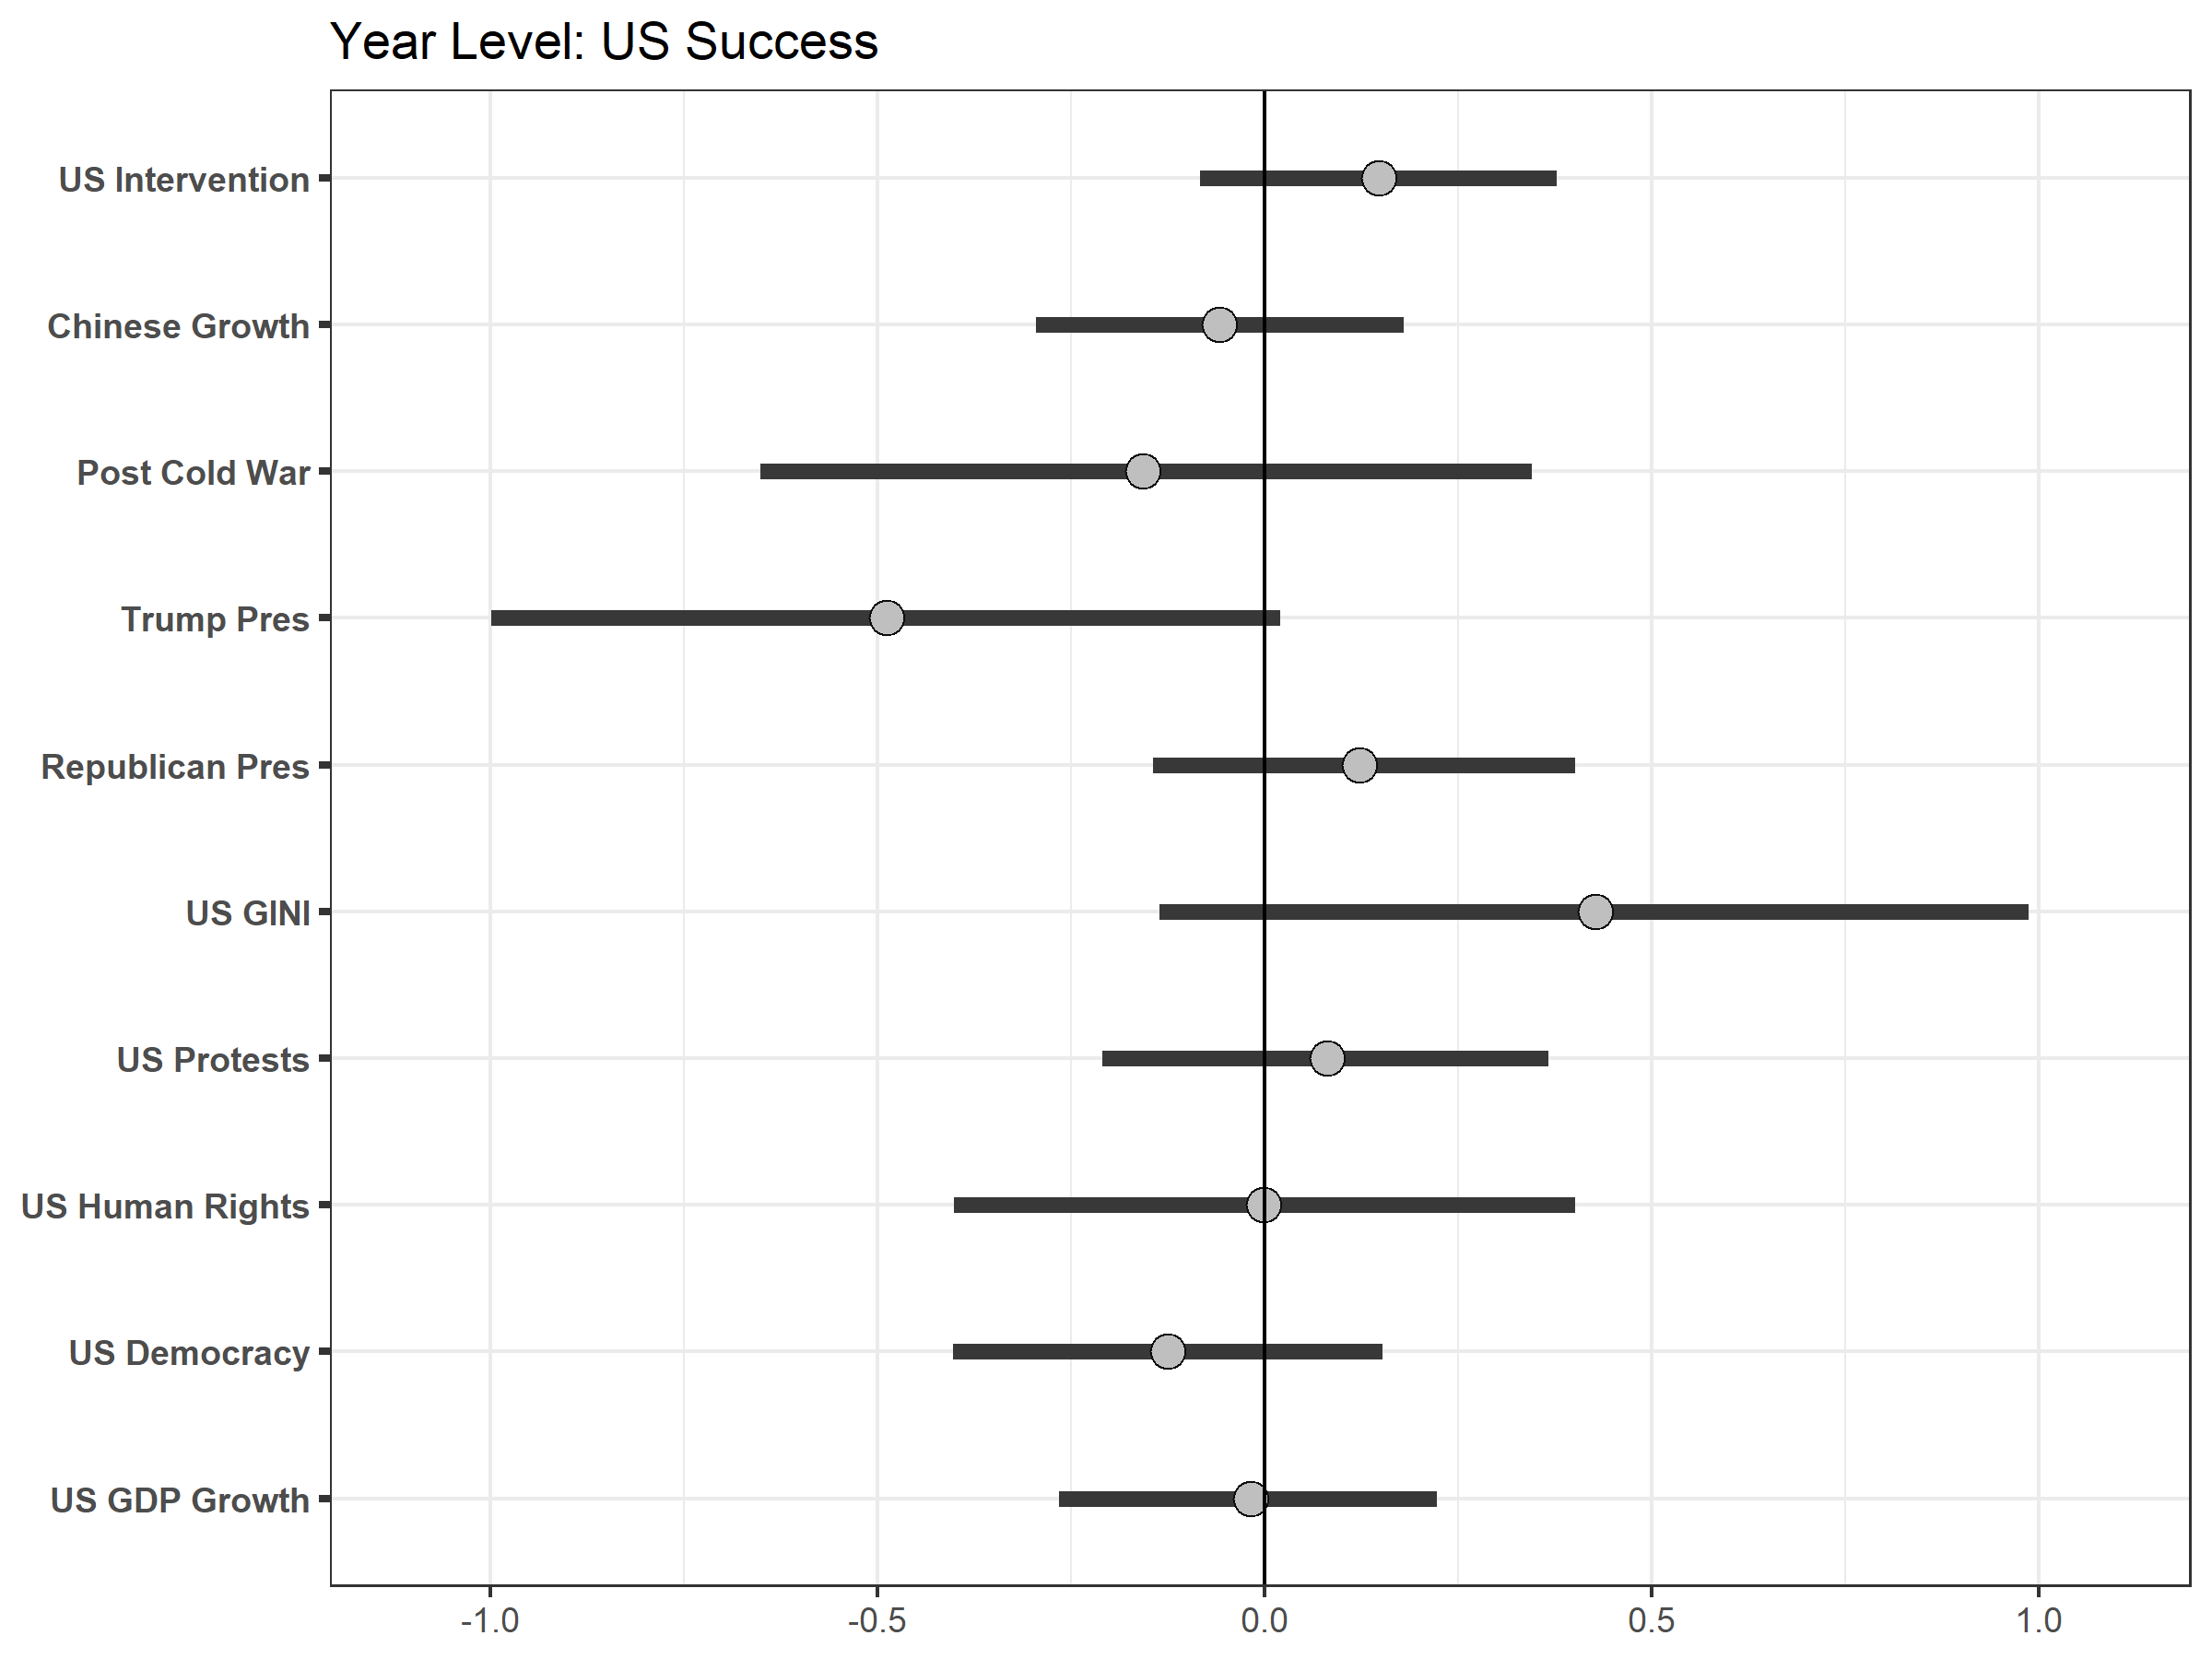
\includegraphics[width = .95\textwidth]{year-var-indiv.png}
\caption{Year-level regression parameters in a multilevel model of foreign attitudes towards democracy and U.S. success, 1980 to 2019. In this model individual-level slopes vary by country. Points mark the posterior median, and the error bars summarize the 90\% credible interval.}
\label{fig:year-var-indiv} 
\end{figure}
  
  
  \newpage
\bibliography{../../MasterBibliography} 




\end{document}
